The training data consists of one hundred silicate samples with the following setup: 
\begin{enumerate}
    \item Dry (vacuum), free surfaces in two directions.
    \item Wet (H20 in voids), free surfaces in two directions
    \item Dry (vacuum), fully periodic (toroidal) boundary conditions.
    \item Wet (H20 in voids), fully periodic (toroidal) boundary conditions.
\end{enumerate}

The silicate is exposed to these conditions following uniform quenching process done at 3.7K/picoseconds. So although we have four different environmental conditions, the procedures starts at equilibrium.
Each instance will contain snapshots of the atoms through time as well as information regarding charge, stress tensor and bond connectivity. 

Molecular dynamics (MD) simulations have shown that silicates that have their fracture regions contacted with an aqueous environment have their Si-O bond energy threshold lowered by 25$\%$  \cite{chem_effects}. Since there are?is? both mechanical loading (stress) and chemical that affect the crack tips, it becomes more difficult to predict fracture propagation. Running simulations of the chemical-mechanical effects on crack tips showed differing rates of fracture propagation as well as changes in fracture direction and even stress distribution in the atoms in the fracture process zone. 

\begin{comment}
\begin{figure}[!b]
  \centering
  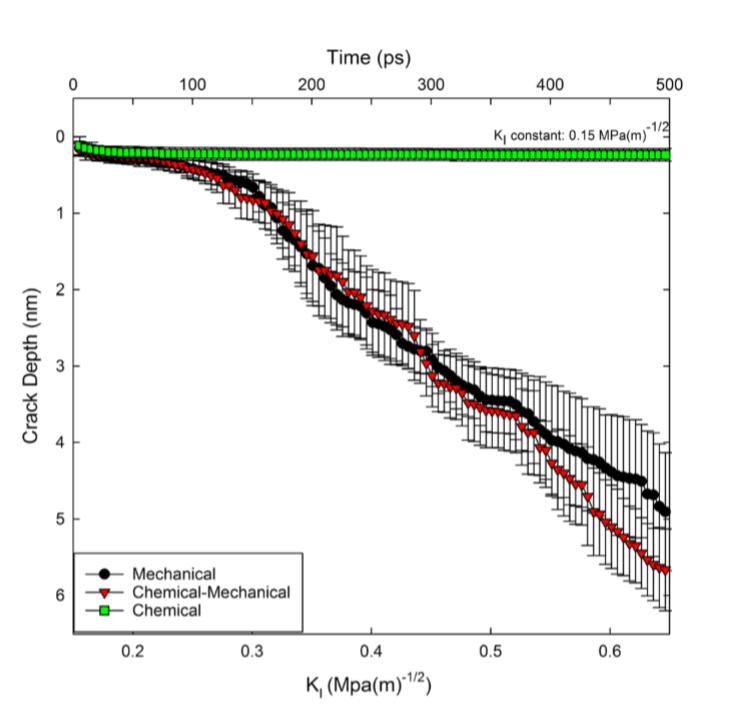
\includegraphics[width=11cm]{picture/crack_depth.PNG}
  \caption{Crack depth for silica systems under mechanical, chemical, and chemical-mechanical conditions.  Figure reproduced from~\protect\cite{chem_effects}}
  \label{crack_depth}
\end{figure}
\end{comment}

\begin{comment}
\begin{figure}[!b]
  \centering
  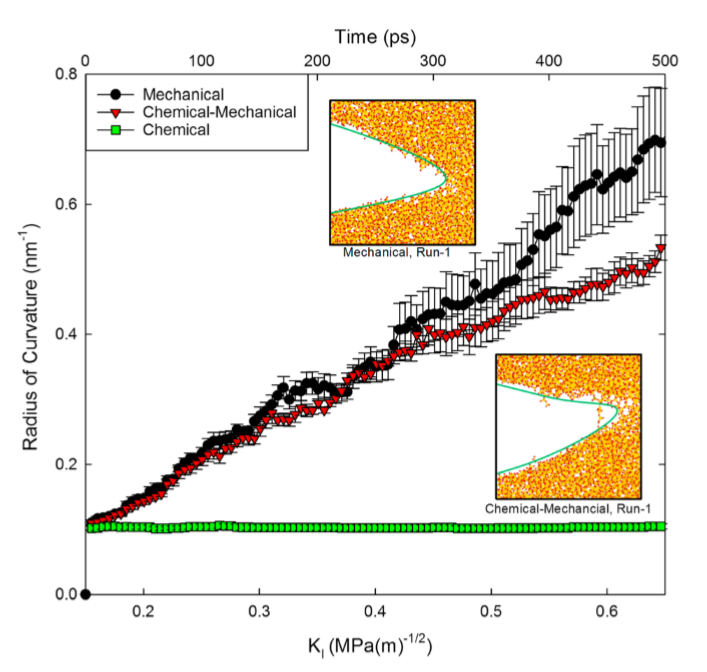
\includegraphics[width=11cm]{picture/crack_radius.PNG}
  \caption{Radius of curavture for silica systems under mechanical, chemical, and chemical-mechanical conditions. Figure reproduced from~\protect\cite{chem_effects}} 
  \label{crack_rad}
\end{figure}
\end{comment}

Therefore, knowing the initial conditions of the silicate glass environment is critical in predicting fracture behavior and  will test the robustness of our model.

\begin{comment}
\begin{figure}[ht]
    \centering
    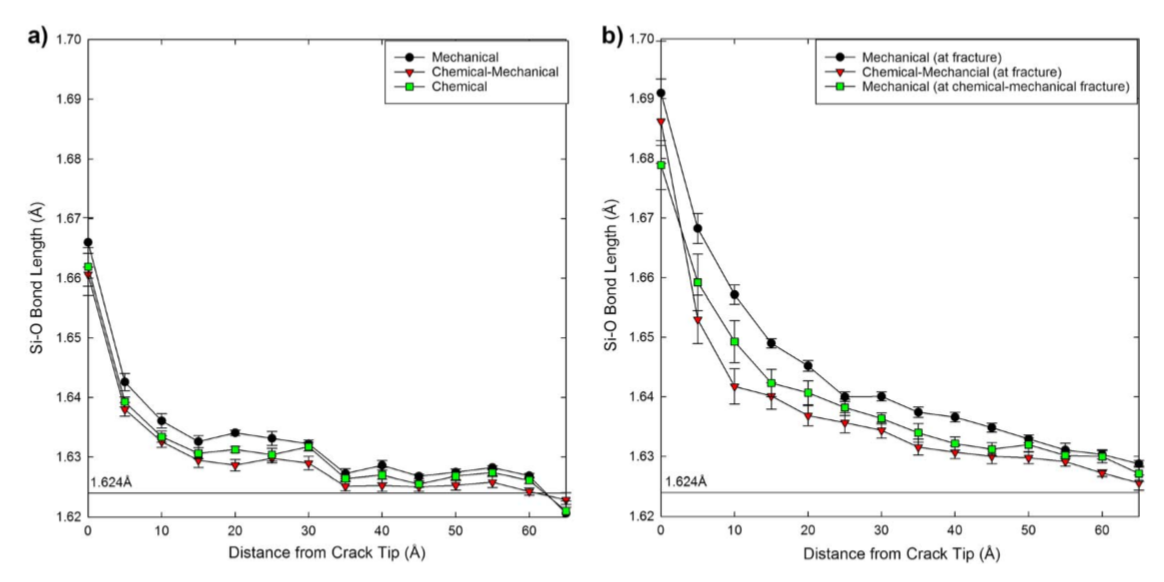
\includegraphics[width=10cm]{picture/AverageSiO.PNG}
    \caption{Average Si─O bond length based on distance from the crack tip at (a) initial conditions and (b) after loading.}
    \label{Average Si-O}
\end{figure}
\end{comment}


